\documentclass[12pt,space]{ctexart} %ans
\usepackage{GKExam}
\usepackage{tikz}
\usepackage{graphicx}
\usepackage{float}
\usepackage{caption}

\usetikzlibrary{positioning, shapes.geometric}
\begin{document}\zihao{5}
\juemi% 输出绝密
\biaoti{2016年普通高等学校招生全国统一考试}
\fubiaoti{上海\hspace{2em}数学试卷(理工农医类)}
{\heiti 考生注意:}
\begin{enumerate}[itemsep=-0.3em,topsep=0pt]
\item 本试卷共 \pageref{LastPage} 页,23道试题,满分为150分,考试时间为120分钟.
\item 本考试分设试卷和答题纸. 试卷包括试题与答题要求. 作答必须涂(选择题)或写(非选择题)在答题纸上,在试卷上作答一律不得分.
\item 答卷前,务必用钢笔或圆珠笔在答题纸正面清楚地填写名字、准考证号,并将核对后的条形码贴在指定位置上,在答题纸反面清楚地填写名字.
\end{enumerate}

\section{填空题(本大题共有14题,满分56分)考生应在答题纸相应编号的空格内直接填写结果,每个空格填对得4分,否则一律得零分.}
\begin{enumerate}[itemsep=-0.3em,topsep=0pt]

  \item 设$x\in R$,则不等式$|x-3|<1$的解集为\blank{$(2,4)$}.
  \item 设$\displaystyle{z=\frac{3+2i}{i}}$,其中$i$为虚数单位,则$\text{Im} z=$\blank{-3}.
  \item 已知平行直线$l_1: 2x+y-1=0$,$l_2: 2x+y+1=0$,则$l_1$,$l_2$的距离\blank{$\frac{2\sqrt{5}}{5}$}.
  \item 某次体检,6位同学的身高(单位:米)分别为1.72,1.78,1.75,1.80,1.69,1.77则这组数据的中位数是\blank{$1.77$}(米).
  \item 已知点$(3,9)$在函数$f(x)=1+a^x$的图像上,则$f(x)$的反函数$f^{-1}(x)=$\blank{$log_2(x-1)$}.
  \item 如图,在正四棱柱$ABCD-A_1B_1C_1D_1$中,底面$ABCD$的边长为3,$BD_1$与底面所成角的大小为$\displaystyle{\arctan{\frac{2}{3}}}$,
        则该正四棱柱的高等于\blank{$2\sqrt{2}$}.
  \item 方程$3\sin x=1+\cos 2x$在区间$[0,2\pi]$上的解为\blank{$30^{\circ}$或$150^{\circ}$}.
  \item 在$\displaystyle{\left (\sqrt[3]{x}-\frac{2}{x}\right )^n}$的二项式中,所有项的二项式系数之和为256,则常数项等于\blank{112}.
  \item 已知$\triangle ABC$的三边长分别为3,5,7,则该三角形的外接圆半径等于\blank{$\frac{7\sqrt{3}}{3}$}.
  \item 设$a>0$,$b>0$,若关于$x$,$y$的方程组$\begin{cases}ax+y=1\\x+by=1\end{cases}$无解,则$a+b$的取值范围是\blank{$[2,+\infty)$}.
  \item 无穷数列$\{a_n\}$由$k$个不同的数组成,$S_n$为$\{a_n\}$的前$n$项和. 若对任意$n\in N^*$,$S_n\in \{2,3\}$,则$k$的最大值为\blank{$4$}.
  \item 在平面直角坐标系中,已知$A(1,0)$,$B(0,-1)$,$P$是曲线$y=\sqrt{1-x^2}$上一个动点,
        则$\overrightarrow{BP}\cdot \overrightarrow{BA}$的取值范围是\blank{$[0,1+\sqrt{2}]$}.
  \item 设$a,b\in R$,$c\in [0,2\pi)$,若对任意实数$x$都有$\displaystyle{2\sin\left (3x-\frac{\pi}{3}\right )=a\sin(bx+c)}$,
        则满足条件的有序实数组$(a,b,c)$的组数为\blank{4}.

  \begin{minipage}[h][4em][t]{.7\textwidth}
    \item 如图,在平面直角坐标系$xOy$中,$O$为正八边形$A_1A_2\cdots A_8$的中心,$A_1(1,0)$. 任取不同的两点$A_i$,$A_j$,
    $P$ 满足 $\overrightarrow{OP} + \overrightarrow{OA_i} + \overrightarrow{OA_j} = \overrightarrow{0}$,
    则点$P$落在第一象限的概率是\blank{Unknown}.
  \end{minipage}
  \begin{minipage}[h][35pt][t]{.25\textwidth}
    \centering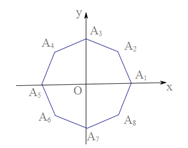
\includegraphics[width=0.8\textwidth]{Image/sh-14.png}
  \end{minipage}

\end{enumerate}

\section{选择题(本大题共有4题,满分20分)}
\begin{enumerate}[itemsep=-0.3em,topsep=0pt, resume]

  \item 设$\alpha\in R$,则“$\alpha>1$”是“$\alpha^2>1$”的
  \begin{tasks}(2)
    \task 充分非必要条件 \task 必要非充分条件 \task 充要条件 \task 既非充分也非必要条件
  \end{tasks}\vspace{1em}
  
  \begin{minipage}[h][5em][t]{.6\textwidth}
    \item 下列极坐标方程中,对应的曲线为右图的是
    \begin{tasks}(2)
      \task $\rho=6+5\cos\theta$ \task $\rho=6+5\sin\theta$ \task $\rho=6-5\cos\theta$ \task $\rho=6-5\sin\theta$
    \end{tasks}
  \end{minipage}
  \begin{minipage}[h][4em][b]{.3\textwidth}
    \centering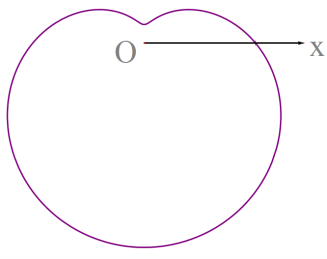
\includegraphics[width=0.45\textwidth]{Image/sh-16.png}
  \end{minipage}

  \item 已知无穷等比数列$\{a_n\}$的公比为$q$,前$n$项和为$S_n$,且$\lim_{n\rightarrow\infty}S_n=S$. 下列条件中,
        使得$2S_n<S\,(n\in N^*)$恒成立的是
  \begin{tasks}(2)
    \task $a_1>0$,$0.6<q<0.7$ \task $a_1<0$,$-0.7<q<-0.6$ 
    \task $a_1>0$,$0.7<q<0.8$ \task $a_1<0$,$-0.8<q<-0.7$ 
  \end{tasks}

  \item 设$f(x)$、$g(x)$、$h(x)$是定义域为$R$的三个函数,对于命题:\ding{172}若$f(x)+g(x)$、$f(x)+h(x)$、$g(x)+h(x)$均为增函数,
        则$f(x)$、$g(x)$、$h(x)$中至少有一个增函数;\ding{173}若$f(x)+g(x)$、$f(x)+h(x)$、$g(x)+h(x)$均是以$T$为周期的函数,
        则$f(x)$、$g(x)$、$h(x)$均是以$T$为周期的函数,下列判断正确的是
  \begin{tasks}(2)
    \task \ding{172}和\ding{173}均为真命题 \task \ding{172}和\ding{173}均为假命题
    \task \ding{172}为真命题,\ding{173}为假命题 \task \ding{172}为假命题,\ding{173}为真命题
  \end{tasks}

\end{enumerate}

\section{解答题(本大题共有5题,满分74分)}
\begin{enumerate}[itemsep=-0.3em,topsep=0pt, resume]

  \item (本题满分12分)\\[0.5em] 
    \begin{minipage}[h][18ex][t]{.63\textwidth}
      如图,将边长为1的正方形$AA_1O_1O$(及其内部)绕的$OO_1$旋转一周形成圆柱,$AC$长为$\displaystyle{\frac 23\pi}$,$A_1B_1$长为$\displaystyle{\frac 13\pi}$,
      其中$B_1$与$C$在平面$AA_1O_1O$的同侧. 
      \begin{enumerate}[itemsep=-0.3em,label={(\arabic*)},topsep=0pt,labelsep=.5em,leftmargin=1.7em]
        \item 求三棱锥$C-O_1A_1B_1$的体积;
        \item 求异面直线$B_1C$与$AA_1$所成的角的大小. 
      \end{enumerate}
    \end{minipage}
    \begin{minipage}[h][18ex][b]{.35\textwidth}
      \begin{figure}[H]
        \centering
        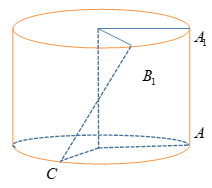
\includegraphics[width=0.7\textwidth]{Image/sh-19.png}
      \end{figure}
    \end{minipage}

    \item (本题满分14分)\\[0.5em] 
    \begin{minipage}[h][16em][t]{.63\textwidth}
      如图,有一块正方形菜地$EFGH$,$EH$所在直线是一条小河,收货的蔬菜可送到$F$点或河边运走. 于是,菜地分为两个区域$S_1$和$S_2$,其中$S_1$中的蔬菜运到河边较近,
      $S_2$中的蔬菜运到$F$点较近,而菜地内$S_1$和$S_2$的分界线$C$上的点到河边与到$F$点的距离相等,现建立平面直角坐标系,其中原点$O$为$EF$的中点,
      点$F$的坐标为$(1,0)$
      \begin{enumerate}[itemsep=-0.3em,label={(\arabic*)},topsep=0pt,labelsep=.5em,leftmargin=1.7em]
        \item 求菜地内的分界线$C$的方程;
        \item 菜农从蔬菜运量估计出$S_1$面积是$S_2$面积的两倍,由此得到$S_1$面积的“经验值”为$\displaystyle{\frac 38}$. 设$M$是$C$上纵坐标为1的点,
              请计算以$EH$为一边、另一边过点$M$的矩形的面积,及五边形$EOMGH$的面积,并判断哪一个更接近于$S_1$面积的“经验值”. 
      \end{enumerate}
    \end{minipage}
    \begin{minipage}[h][9em][b]{.35\textwidth}
      \begin{figure}[H]
        \centering
        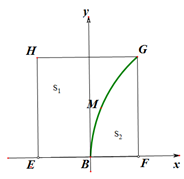
\includegraphics[width=0.8\textwidth]{Image/sh-20.png}
      \end{figure}
    \end{minipage}

    \item (本题满分14分)\\
    双曲线$\displaystyle{x^2-\frac{y^2}{b^2}=1\,(b>0)}$的左、右焦点分别为$F_1$、$F_2$,直线$l$过$F_2$且与双曲线交于$A$、$B$两点. 
    \begin{enumerate}[itemsep=-0.3em,label={(\arabic*)},topsep=0pt,labelsep=.5em,leftmargin=1.7em]
      \item 若$l$的倾斜角为$\displaystyle{\frac{\pi}{2}}$,$\triangle F_1AB$是等边三角形,求双曲线的渐近线方程;
      \item 设$b=\sqrt{3}$,若$l$的斜率存在,且$(\overrightarrow{F_1A}+\overrightarrow{F_1B})\cdot\overrightarrow{AB}=0$,求$l$的斜率.
    \end{enumerate}

    \item (本题满分16分)\\
    已知$a\in R$,函数$\displaystyle{f(x)=\log_2(\frac{1}{x}+a)}$.
    \begin{enumerate}[itemsep=-0.3em,label={(\arabic*)},topsep=0pt,labelsep=.5em,leftmargin=1.7em]
      \item 当$a=5$时,解不等式$f(x)>0$;
      \item 若关于$x$的方程$f(x)-log_2[(a-4)x+2a-5]=0$的解集中恰好有一个元素,求$a$的取值范围;
      \item 设$a>0$,若对任意$\displaystyle{t\in [\frac{1}{2}, 1]}$,函数$f(x)$在区间$[t, t+1]$上的最大值与最小值的差不超过1,求$a$的取值范围.
    \end{enumerate}

    \item (本题满分18分)\\
    若无穷数列$\{a_n\}$满足:只要$a_p=a_q\,(p,q\in N^*)$,必有$a_{p+1}=a_{q+1}$,则称$\{a_n\}$具有性质$P$.
    \begin{enumerate}[itemsep=-0.3em,label={(\arabic*)},topsep=0pt,labelsep=.5em,leftmargin=1.7em]
      \item 若$\{a_n\}$具有性质$P$,且$a_1=1$,$a_2=2$,$a_4=3$,$a_5=2$,$a_6+a_7+a_8=21$. 求$a_3$;
      \item 若无穷数列$\{b_n\}$是等差数列,无穷数列$\{c_n\}$是公比为正数的等比数列,$b_1=c_5=1$,$b_5=c_1=81$,$a_n=b_n+c_n$.
            判断$\{a_n\}$是否具有性质$P$,并说明理由;
      \item 设$\{b_n\}$是无穷数列,已知$a_{n+1}=b_n+\sin a_n\,(n\in N^*)$. 求证:“对任意$a_1$都具有性质$P$”的充要条件为“$\{b_n\}$是常数列”.
    \end{enumerate}

\end{enumerate}

%%%%%%%%%%%%%%%%%%%%%%%%%%%%%%%%%%%%%%%%%%%%%%%%%%%%%%%%%%%%%%%%%%%%%%%%%%
%---------------------------------结束------------------------------------
%%%%%%%%%%%%%%%%%%%%%%%%%%%%%%%%%%%%%%%%%%%%%%%%%%%%%%%%%%%%%%%%%%%%%%%%%%
\clearpage

\end{document}
